\section{Poly\-Line Class Reference}
\label{classPolyLine}\index{PolyLine@{PolyLine}}
{\tt \#include $<$polyline.h$>$}

Inheritance diagram for Poly\-Line::\begin{figure}[H]
\begin{center}
\leavevmode
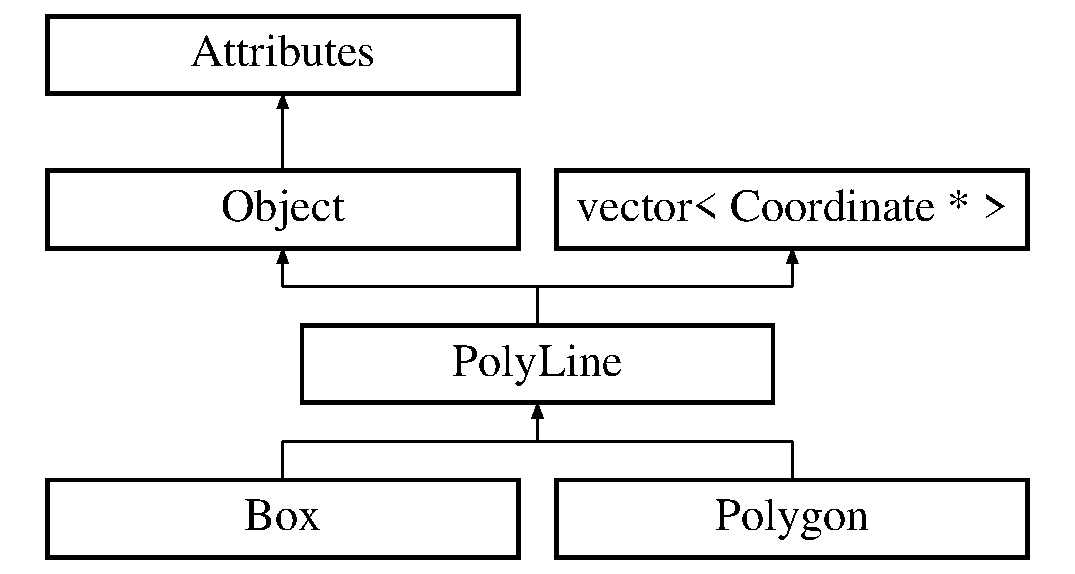
\includegraphics[height=4cm]{classPolyLine}
\end{center}
\end{figure}
\subsection*{Public Types}
\begin{CompactItemize}
\item 
enum {\bf Sub\-Types} \{ {\bf Poly\-Line\-Type} =   1, 
{\bf Box\-Type} =  2, 
{\bf Polygon\-Type} =  3, 
{\bf Arc\-Box\-Type} =  4, 
{\bf Picture\-Type} =  5
 \}
\end{CompactItemize}
\subsection*{Public Methods}
\begin{CompactItemize}
\item 
{\bf Poly\-Line} ()
\item 
{\bf Poly\-Line} ({\bf Coordinate} $\ast$point1, {\bf Coordinate} $\ast$point2)
\item 
{\bf $\sim$Poly\-Line} ()
\item 
int {\bf get\-Sub\-Type} ()
\item 
void {\bf write} (std::ostream \&stream) const
\end{CompactItemize}
\subsection*{Protected Methods}
\begin{CompactItemize}
\item 
void {\bf set\-Sub\-Type} ({\bf Sub\-Types} {\bf sub\-Type})
\end{CompactItemize}
\subsection*{Private Attributes}
\begin{CompactItemize}
\item 
{\bf Sub\-Types} {\bf sub\-Type}
\end{CompactItemize}


\subsection{Detailed Description}
This class handles polyline objects. This class is derived from {\bf Object} {\rm (p.\,\pageref{classObject})}. It acts as a vector (C++ standard library) container for instances of {\bf Coordinate} {\rm (p.\,\pageref{classCoordinate})} \begin{Desc}
\item[Author: ]\par
Anthony Liekens \end{Desc}




\subsection{Member Enumeration Documentation}
\index{PolyLine@{Poly\-Line}!SubTypes@{SubTypes}}
\index{SubTypes@{SubTypes}!PolyLine@{Poly\-Line}}
\subsubsection{\setlength{\rightskip}{0pt plus 5cm}enum Poly\-Line::Sub\-Types}\label{classPolyLine_s5}


Enumeration of polyline types. The following types can be used to set the type of a polyline object : \{$\backslash$tt Poly\-Line\-Type, Box\-Type, Polygon\-Type, Picture\-Type\}. Inherited polyline classes will set their appropriate type. \begin{Desc}
\item[Enumeration values: ]\par
\begin{description}
\index{PolyLineType@{PolyLineType}!PolyLine@{PolyLine}}\index{PolyLine@{PolyLine}!PolyLineType@{PolyLineType}}\item[{\em 
{\em Poly\-Line\-Type}\label{classPolyLine_s5s0}
}]\index{BoxType@{BoxType}!PolyLine@{PolyLine}}\index{PolyLine@{PolyLine}!BoxType@{BoxType}}\item[{\em 
{\em Box\-Type}\label{classPolyLine_s5s1}
}]\index{PolygonType@{PolygonType}!PolyLine@{PolyLine}}\index{PolyLine@{PolyLine}!PolygonType@{PolygonType}}\item[{\em 
{\em Polygon\-Type}\label{classPolyLine_s5s2}
}]\index{ArcBoxType@{ArcBoxType}!PolyLine@{PolyLine}}\index{PolyLine@{PolyLine}!ArcBoxType@{ArcBoxType}}\item[{\em 
{\em Arc\-Box\-Type}\label{classPolyLine_s5s3}
}]\index{PictureType@{PictureType}!PolyLine@{PolyLine}}\index{PolyLine@{PolyLine}!PictureType@{PictureType}}\item[{\em 
{\em Picture\-Type}\label{classPolyLine_s5s4}
}]\end{description}
\end{Desc}



\subsection{Constructor \& Destructor Documentation}
\index{PolyLine@{Poly\-Line}!PolyLine@{PolyLine}}
\index{PolyLine@{PolyLine}!PolyLine@{Poly\-Line}}
\subsubsection{\setlength{\rightskip}{0pt plus 5cm}Poly\-Line::Poly\-Line ()}\label{classPolyLine_a0}


Constructor. Constructs a polyline object \index{PolyLine@{Poly\-Line}!PolyLine@{PolyLine}}
\index{PolyLine@{PolyLine}!PolyLine@{Poly\-Line}}
\subsubsection{\setlength{\rightskip}{0pt plus 5cm}Poly\-Line::Poly\-Line ({\bf Coordinate} $\ast$ {\em point1}, {\bf Coordinate} $\ast$ {\em point2})}\label{classPolyLine_a1}


Constructor. Constructs a polyline object with 2 points \begin{Desc}
\item[Parameters: ]\par
\begin{description}
\item[{\em 
point1}]- Instance of {\bf Coordinate} {\rm (p.\,\pageref{classCoordinate})}. Coordinates of the first point \item[{\em 
point2}]- Instance of {\bf Coordinate} {\rm (p.\,\pageref{classCoordinate})}. Coordinates of the second point \end{description}
\end{Desc}
\index{PolyLine@{Poly\-Line}!~PolyLine@{$\sim$PolyLine}}
\index{~PolyLine@{$\sim$PolyLine}!PolyLine@{Poly\-Line}}
\subsubsection{\setlength{\rightskip}{0pt plus 5cm}Poly\-Line::$\sim$Poly\-Line ()}\label{classPolyLine_a2}


Destructor. Destructs a polyline object 

\subsection{Member Function Documentation}
\index{PolyLine@{Poly\-Line}!getSubType@{getSubType}}
\index{getSubType@{getSubType}!PolyLine@{Poly\-Line}}
\subsubsection{\setlength{\rightskip}{0pt plus 5cm}int Poly\-Line::get\-Sub\-Type ()\hspace{0.3cm}{\tt  [inline]}}\label{classPolyLine_a3}


Returns the polyline sub type \begin{Desc}
\item[Returns: ]\par
Instance of {\bf Sub\-Types} {\rm (p.\,\pageref{classPolyLine_s5})} \end{Desc}
\index{PolyLine@{Poly\-Line}!setSubType@{setSubType}}
\index{setSubType@{setSubType}!PolyLine@{Poly\-Line}}
\subsubsection{\setlength{\rightskip}{0pt plus 5cm}void Poly\-Line::set\-Sub\-Type ({\bf Sub\-Types} {\em sub\-Type})\hspace{0.3cm}{\tt  [inline, protected]}}\label{classPolyLine_b0}


Set the sub type \begin{Desc}
\item[Parameters: ]\par
\begin{description}
\item[{\em 
sub\-Type}]{\bf Sub\-Types} {\rm (p.\,\pageref{classPolyLine_s5})} \end{description}
\end{Desc}
\begin{Desc}
\item[Returns: ]\par
void \end{Desc}
\index{PolyLine@{Poly\-Line}!write@{write}}
\index{write@{write}!PolyLine@{Poly\-Line}}
\subsubsection{\setlength{\rightskip}{0pt plus 5cm}void Poly\-Line::write (std::ostream \& {\em stream}) const\hspace{0.3cm}{\tt  [virtual]}}\label{classPolyLine_a4}


Write the polyline object to a given outstream. \begin{Desc}
\item[Parameters: ]\par
\begin{description}
\item[{\em 
stream}]output stream \end{description}
\end{Desc}
\begin{Desc}
\item[Returns: ]\par
void \end{Desc}


Reimplemented from {\bf Object} {\rm (p.\,\pageref{classObject_a3})}.

\subsection{Member Data Documentation}
\index{PolyLine@{Poly\-Line}!subType@{subType}}
\index{subType@{subType}!PolyLine@{Poly\-Line}}
\subsubsection{\setlength{\rightskip}{0pt plus 5cm}{\bf Sub\-Types} Poly\-Line::sub\-Type\hspace{0.3cm}{\tt  [private]}}\label{classPolyLine_o0}




The documentation for this class was generated from the following files:\begin{CompactItemize}
\item 
{\bf polyline.h}\item 
{\bf polyline.cpp}\end{CompactItemize}
